\chapter{Enqu\^ete}
    \label{enqueteappendix}
      \section{Demografie}
        Om te kijken in hoeverre de enqu\^ete de mening van alle Wakoopa-leden vertegenwoordigd, is het belangrijk om te kijken of de demografie van de twee overeenkomen. De demografie van de respondenten is te vinden in figuren \ref{fig:gender}, \ref{fig:country} en \ref{fig:age}. Qua leeftijd, geslacht en land verschilt dit slechts een aantal procenten met de demografie van Wakoopa-gebruikers. De enqu\^ete, met 1069 respondenten, is daarom een goede graadmeter van de mening van Wakoopa-leden.
        \begin{figure}
          \begin{center}
          \caption{Geslacht van respondenten}
            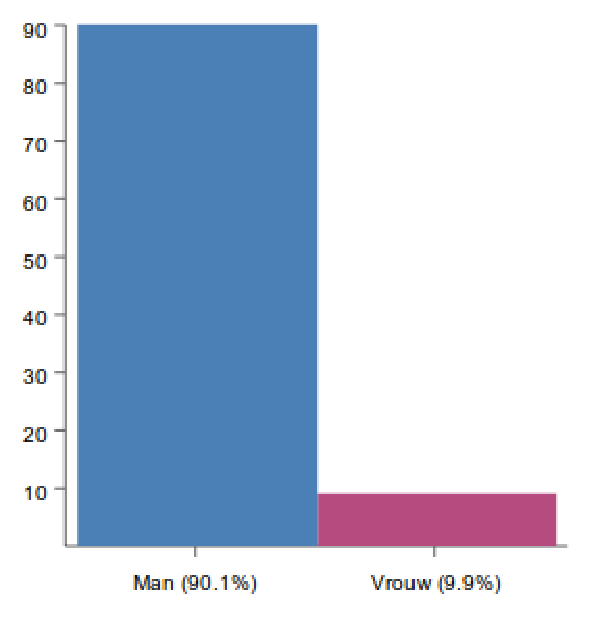
\includegraphics[height=60mm, angle=90]{../images/enquete/gender}
          \label{fig:gender}

          \caption{Land van afkomst van respondenten}
            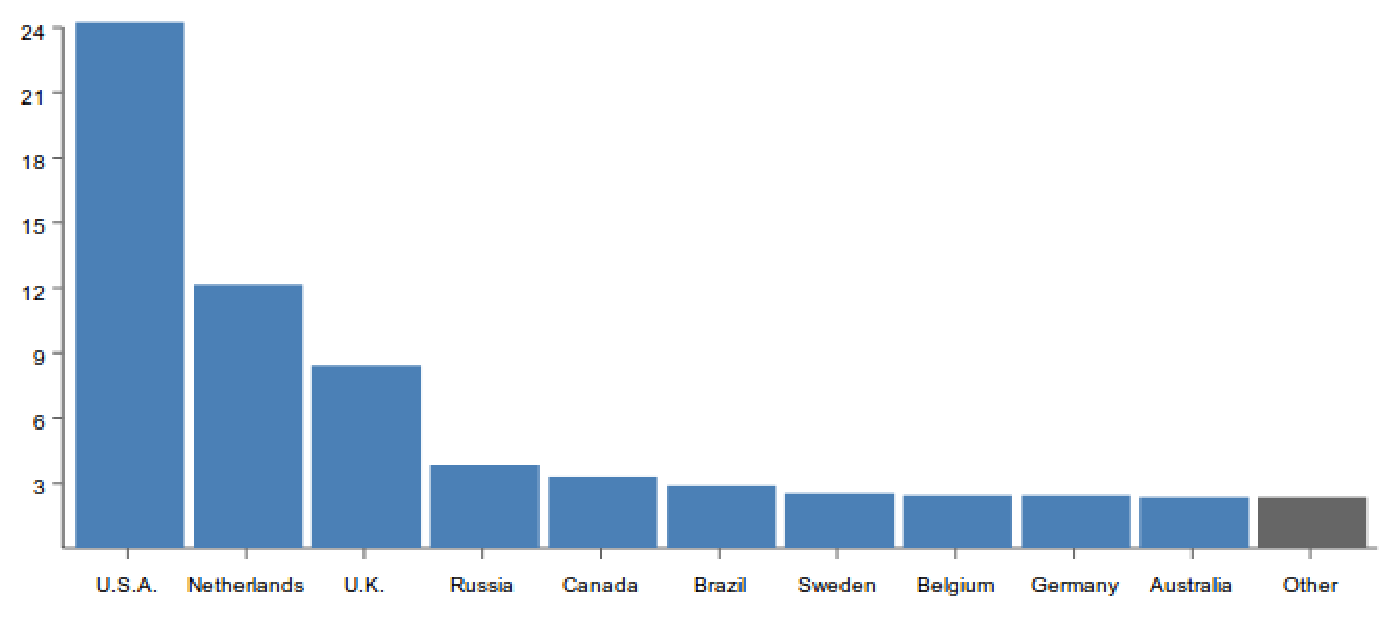
\includegraphics[height=60mm, angle=90]{../images/enquete/country}
            \label{fig:country}

          \end{center}
        \end{figure}

        \begin{figure}
          \begin{center}
          \caption{Leeftijd van respondenten}
            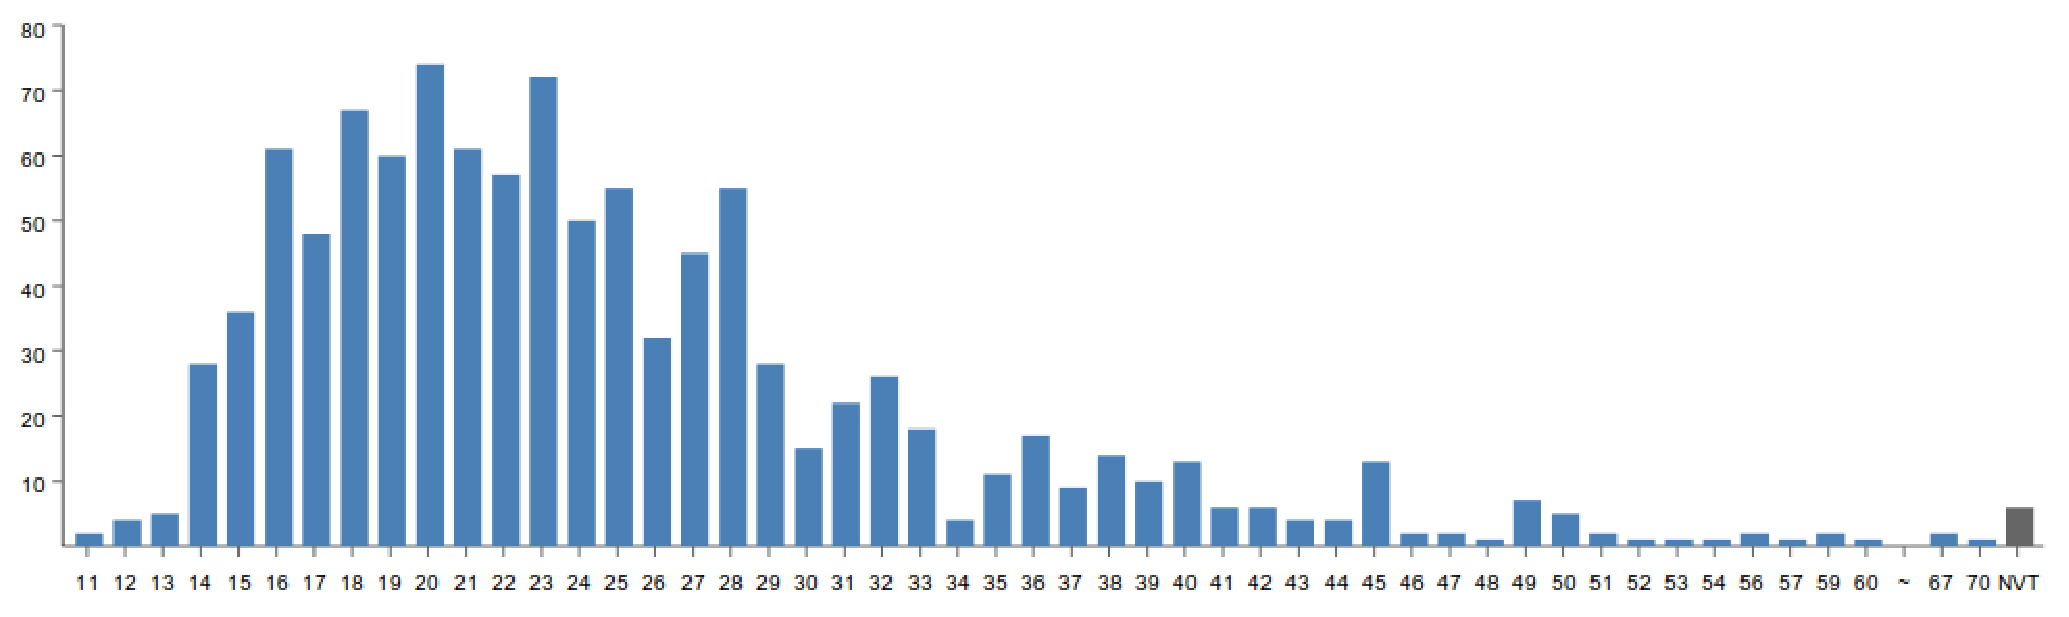
\includegraphics[height=58mm, angle=90]{../images/enquete/age}
          \label{fig:age}

          \end{center}
        \end{figure}

      \section{Bevindingen}
        De enqu\^ete ging verder met vragen naar hoe kundig de respondenten met computers waren (Figuur \ref{fig:skill}). Het overgrote deel (49.2\%) van de respondenten vind zichzelf \emph{excellent} op computergebied. Een klein percentage vind zichzelf een novice (0.3\%) of classificeerd zichzelf als `lerende' (1.5\%). Eenentwintig procent acht zichzelf in het midden met `pretty good'. Als laatste is achtentwintig procent van de respondenten zelf actief bezig met het ontwikkelen van applicaties. Uit deze uitkomst is op te maken dat zich onder de respondenten een hoog percentage experts, of zogenaamde `power users', bevinden.
        \begin{figure}
          \begin{center}
          \caption{Kundigheid met computers}
            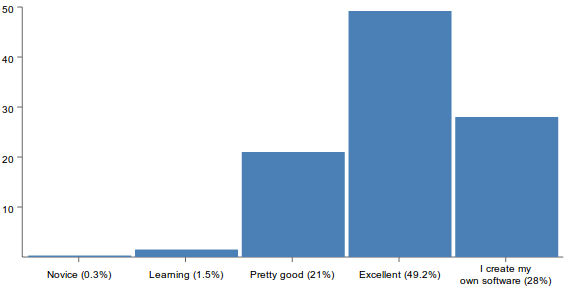
\includegraphics[height=50mm]{../images/enquete/good-with-computers}
          \label{fig:skill}
          \end{center}
        \end{figure}

      In Figuur \ref{fig:visit-website} werd de vraag gesteld hoe vaak gebruikers de Wakoopa site bezochten en er werd gevraagd waarom ze met dit interval de site bekeken. Het overgrote deel --- 43.1\% --- van de respondenten bekeek de site wekelijks, gevolgd door een derde van de respondenten die dagelijks keek. Een greep uit de gegeven redenen:
        \begin{figure}
          \begin{center}
          \caption{Hoe vaak wordt de website bezocht?}
            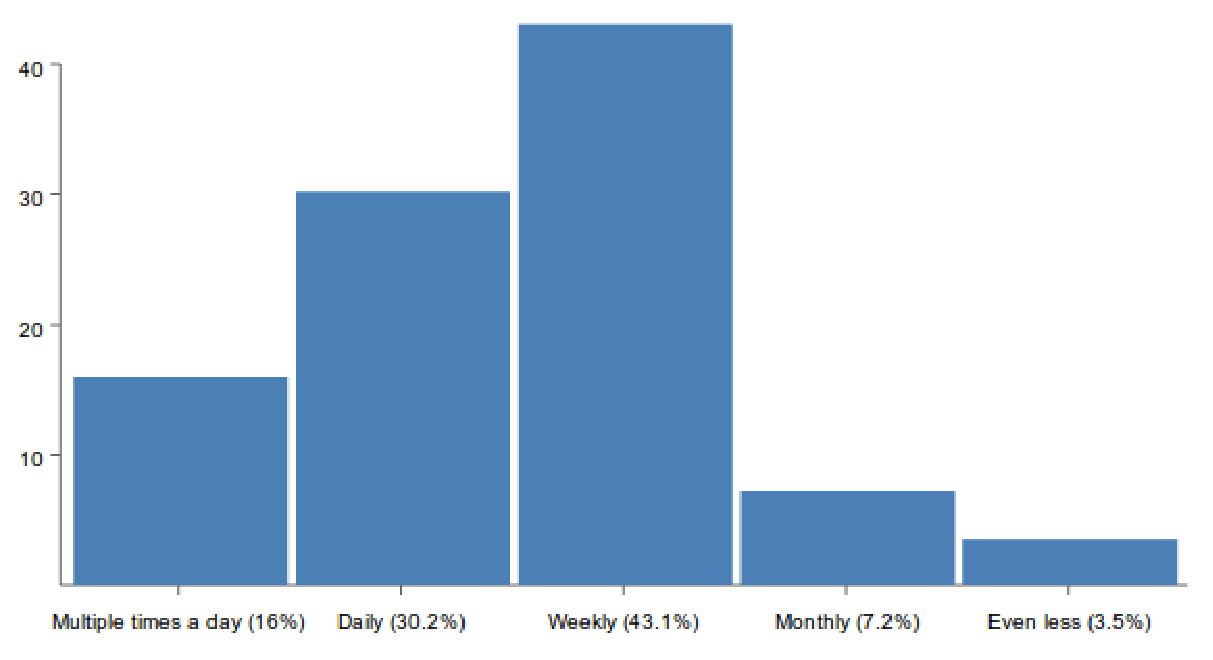
\includegraphics[height=50mm]{../images/enquete/visit-website}
          \label{fig:visit-website}
          \end{center}
        \end{figure}

      \paragraph{Wekelijk (43.1\%)}
        \begin{itemize}
          \item Because of the weekly summary mail
          \item Because that is when I get my summary
          \item I need some weekly reports about my software and timetracking reports.
          \item To see the "big" changes is my software behaviour. And to see if there is new software i could try out.
        \end{itemize}

      \paragraph{Dagelijks (30.2\%)}
        \begin{itemize}
          \item It's interesting to see all the data and usage stuff.
          \item To check what level I am. Always seeking to level up..!
          \item To check out what new software is out there \& it's cool to see what my habits are on my Mac.
          \item Check my profile stats
        \end{itemize}

      \paragraph{Meerdere malen per dag (16\%)}
        \begin{itemize}
          \item To see how many points i'm earning, and to just snoop on other peoples profiles. you know, creep. like on facebook. but the people here are more interesting than my facebook people :)
          \item Well, the system tray icon keeps notifying me the new activities
          \item To see how my friends are doing and me, and so I can win in the battle of using the most software in less time. :)
          \item Because I love statistics, I find it rewarding to see figures and graphs about something I accomplished! that's the reason why I'm also a last.fm and whatpulse addict. and apart from that, I really like software (especially freeware) and like to see suggestions for other software.
        \end{itemize}

      \paragraph{Maandelijks (7.2\%)}
        \begin{itemize}
          \item There's no need to use it more often
          \item Because I got an update.
          \item I like to see my stats and get new ideas on software/sites.
          \item I only check the site when I am looking for alternative software or I see something I like in the newsletter.
        \end{itemize}

      \paragraph{Minder dan maandelijks (3.5\%)}
        \begin{itemize}
          \item I'm still waiting for the linux app
          \item Nothing of tons of interest on site, just as often as I visit Last.FM It is useful when uninstalling things.
          \item Because I use Linux, I am waiting for a Linux tracker. Without it, Wakoopa is just another computer-oriented forum to me.
        \end{itemize}

      \paragraph{}Zoals uit de verschillende gegeven redenen op te merken is, is er een relatie tussen hoe vaak mensen de site bezoeken en hoe enthousiast ze er over zijn. Onder wekelijkse bezoekers is het aantal wat aangeeft de website te bezoeken na het ontvangen van de wekelijkse mail het hoogst. De mensen die een of meerdere malen per dag de site bekijken, zijn er voornamelijk voor de grafieken, statistieken en punten. Omgekeerd, de respondenten die slechts maandelijks of minder de site bekijken, zeggen dat ze dit doen omdat er niet genoeg nieuws of informatie op de site staat om deze vaker te bezoeken.

        \begin{figure}
          \begin{center}
          \caption{Over welke nieuwe functionaliteit ben je het meest enthousiast?}
            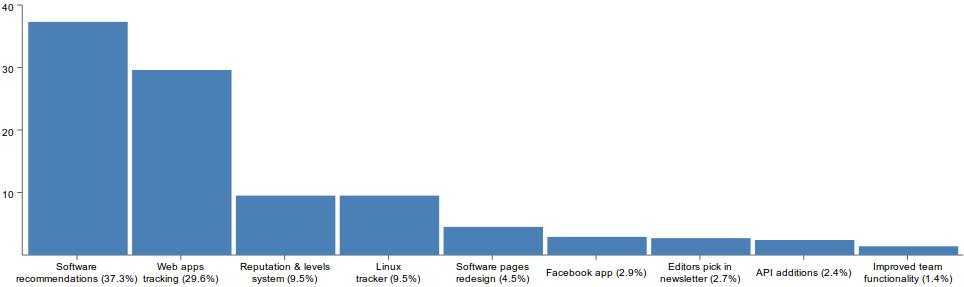
\includegraphics[width=\textwidth]{../images/enquete/recent-additions}
          \label{fig:enthousiast}
          \end{center}
        \end{figure}

      Een learning network is vaak bezig met het ontwikkelen en online plaatsen van nieuwe functionaliteit. Het belangrijk om bij te houden wat de impact hiervan op de gebruikers is. Om dit te onderzoeken vroegen we in figuur \ref{fig:enthousiast} aan de respondenten over welke recente toevoeging ze het meest enthousiast waren. Met 37.3\% zijn de respondenten het meest enthousiast over de software aanbevelingen, kort daarop gevolgd door het tracken van web apps met 29.6\%. De eerstvolgende zijn respectievelijk het level-systeem en de linux tracker met beide 9.5\%.

        \begin{figure}
          \begin{center}
          \caption{Waar komt Wakoopa tekort?}
            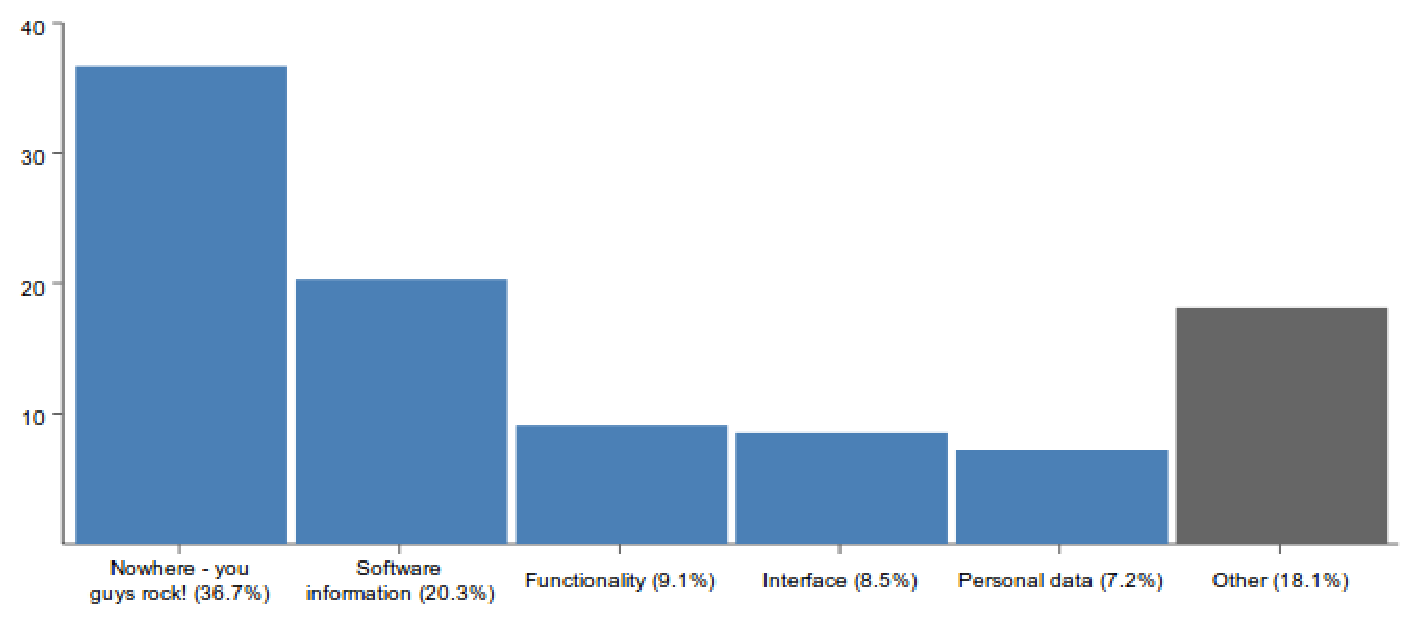
\includegraphics[width=\textwidth]{../images/enquete/improvement}
          \label{fig:improvement}
          \end{center}
        \end{figure}

      Minstens even belangrijk als weten waar mensen enthousiast over zijn is weten waar ze graag verbetering willen zien. Daarom stelde de enqu\^ete de vraag waar de respondenten Wakoopa nog in vonden tekortkomen. De respons hierop is te vinden in figuur \ref{fig:improvement}. Het meest gekozen antwoord was `Nowhere, you guys rock!'. 36.7\% van de respondenten had geen grote problemen, of kon er niet direct een noemen. Hoewel dit positief is, zit de waarde van de vraag meer in de andere antwoorden.

      Een groot deel van de respondenten, 20.3\%, vindt dat de informatie rondom software te wensen overlaat. Een kijk in het help-forum laat zien dat er inderdaad veel mensen toevoegingen aandragen op dit gebied.\footnote{\url{http://getsatisfaction.com/wakoopa/searches?query=software+information&style=topics}, geraadpleegd op 13 oktober 2009} Wat vaak voorkomt zijn vragen over meer informatie qua versies. Een recente ontwikkeling op dit gebied is dat softwareontwikkelaars nu hun versies en downloads op Wakoopa kunnen beheren, en voor een hogere kwaliteit van informatie kunnen zorgen.

      Een ander veelvoorkomend punt is dat mensen graag specifieke informatie vinden, zoals mogelijke problemen of aandachtspunten. Buiten het reviewsysteem, waar mensen ook opmerkingen of problemen in kunnen vermelden, is hier geen mogelijkheid voor, en er wordt geen interface geboden om deze apart van elkaar, of gesorteerd op versie, te bekijken. Zo'n interface zou een waardevolle toevoeging zijn.


      Hierna vonden de respondenten dat de site te kort kwam op algemene functionaliteit (9\%), de interface (8.5\%) en persoonlijke data (7\%) genoemd. 18.1\% kiest voor other, waarbij om een reden werd gevraagd. Hieronder volgt een greep uit de idee\"en van deze responsen:

      \begin{itemize}
      \item Automatic put a message in twitter
      \item You should translate this webpage into other languages. There is no alternative in, for example, Spanish for software recomendation services. It would be the perfect develope for Wakoopa. Conquer the world!
      \item More intuitive tools to compare and analysis statistics about the software listed. This should include the ability to auto-lookup the names of the apps as the name is being typed.
      \item Social network features: I find the current system pointless and that point system made it even worse, I keep seeing people I don't know add me as a contact.
      \item I think the review system could be updated. It seems that a lot of really low quality reviews get in. Perhaps a rating system that the community could use would fix it.
      \item Software Recommendations. On average I seem accumulate 20 PAGES (far too many) of Software Recommendations. Most of which are awful and irrelevant to my usage. Just because I tried a video editor one time doesn't mean I want recommendations for every lame shareware video editor out there. It would be nice if you guys narrowed it down to 10 recommendations based on the top 10 software I use everyday. Right now it feels like spam.
      \end{itemize}

      Kijkende naar deze replies gaan deze vooral over de \emph{interface}, de presentatie of werking van pagina's. Dit zijn concrete punten, zoals bijvoorbeeld het ratingsysteem. Het ratingsysteem op Wakoopa vraagt gebruikers tussen de nul en vijf sterren te geven. Uit statistieken van Youtube\footnote{\url{http://youtube-global.blogspot.com/2009/09/five-stars-dominate-ratings.html}} blijkt dat voor hen dit model niet werkt. Mensen vinden filmpjes goed en geven dan een vijf, of niet goed en nemen niet de moeite om een review te schrijven. Ook op Wakoopa is een soortgelijk patroon te vinden.

      Een usability pattern dat hiermee rekening houdt is het `like' pattern, waar mensen enkel kunnen aangeven of ze iets leuk vinden of niet. Op Wakoopa is sinds dit onderzoek een favoriet-functie toegevoegd die dit like-patroon volgt.

      Links met andere sociale netwerken, het uitzenden van software gebruik naar bijvoorbeeld Facebook of Twitter worden ook meerdere malen genoemd. Buiten een Facebook widget en Friendfeed integratie voldoet Wakoopa nog niet aan deze vraag. Het toevoegen van een `share' knop op softwarepagina's heeft tot weinig extra hits geleid, maar door dit bijvoorbeeld naar `Social' te veranderen, kan door middel van A/B testen worden gekeken of een andere benaming meer effect heeft.

      Een interessant punt is de laatste respons, over het weergeven van minder aanbevelingen. Dit is een paradoxaal punt. Je verwacht dat meer aanbevelingen beter zijn, maar vanuit een gebruikersoogpunt is het wellicht veel interessanter om per categorie een of twee aanbeveling, of een tiental aanbevelingen in totaal te krijgen. Dit cre\"eert het idee dat de aanbevelingen zorgvuldig zijn uitgekozen in plaats van dat er voor alle applicaties wiskundig is gekeken hoeveel het past bij het huidige softwaregebruik van een gebruiker. Omdat de aanbevelingen tweemaal per week veranderen, en er voor wordt gezorgd dat deze niet continue hetzelfde zijn, kan er per week een beperkte set worden weergegeven.

        \begin{figure}
          \begin{center}
          \caption{Wat vinden respondenten van de softwareaanbevelingen?}
            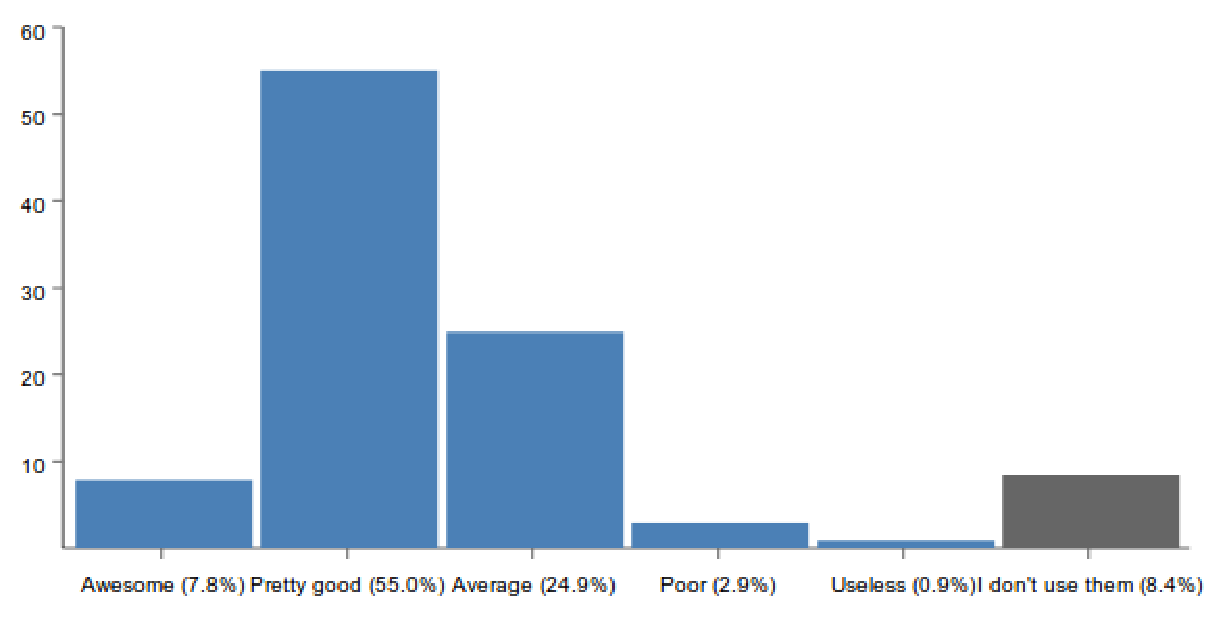
\includegraphics[width=\textwidth]{../images/enquete/think-of-recommendations}
          \label{fig:recommendations}
          \end{center}
        \end{figure}

      \paragraph{}Qua kwaliteit van de aanbevelingen, te zien in figuur \ref{fig:recommendations}, zijn de meeste mensen tevreden. 87.7\% vind de aanbevelingen gemiddeld of bovengemiddeld, en 62.8\% vind ze bovengemiddeld goed. een klein percentage van 8.5\% gebruikt de aanbevelingen in totaal niet. Zoals eerder genoemd zouden we de aanbevelingen exclusiever kunnen laten lijken door er minder tegelijk te laten zien, of per categorie \'e\'en aanbeveling te laten zien.

      Uit figuur \ref{fig:advertisements} blijkt dat het overgrote deel van de respondenten de advertenties niet merken of niet als vervelend ervaren. Deze wetenschap kan een rol spelen bij het plaatsen van advertenties op andere pagina's. Wanneer mensen de advertenties op dit moment niet merken, kunnen deze op een zichtbaardere plaats worden neergezet, wat tot een hogere click-through rate zou moeten leiden.

        \begin{figure}
          \begin{center}
          \caption{Wat vinden respondenten van de advertenties}
            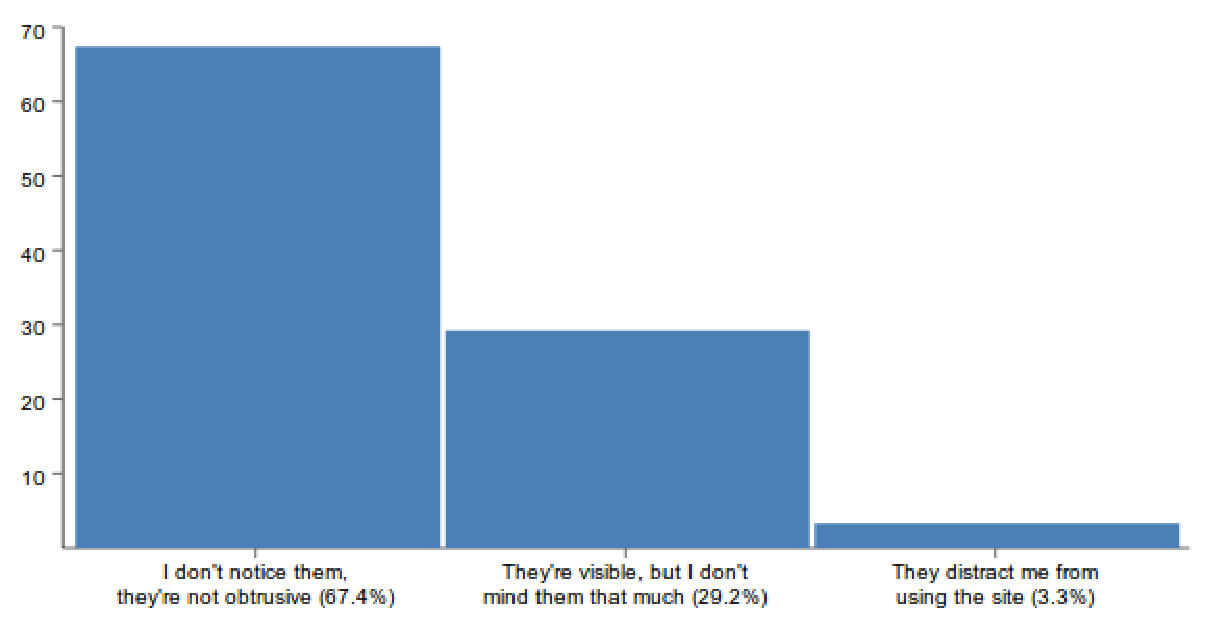
\includegraphics[width=\textwidth]{../images/enquete/advertisements}
          \label{fig:advertisements}
          \end{center}
        \end{figure}

